\section{Matrix$<$ T $>$ Class Template Reference}
\label{classMatrix}\index{Matrix@{Matrix}}
{\tt \#include $<$matrix.h$>$}

Inheritance diagram for Matrix$<$ T $>$::\begin{figure}[H]
\begin{center}
\leavevmode
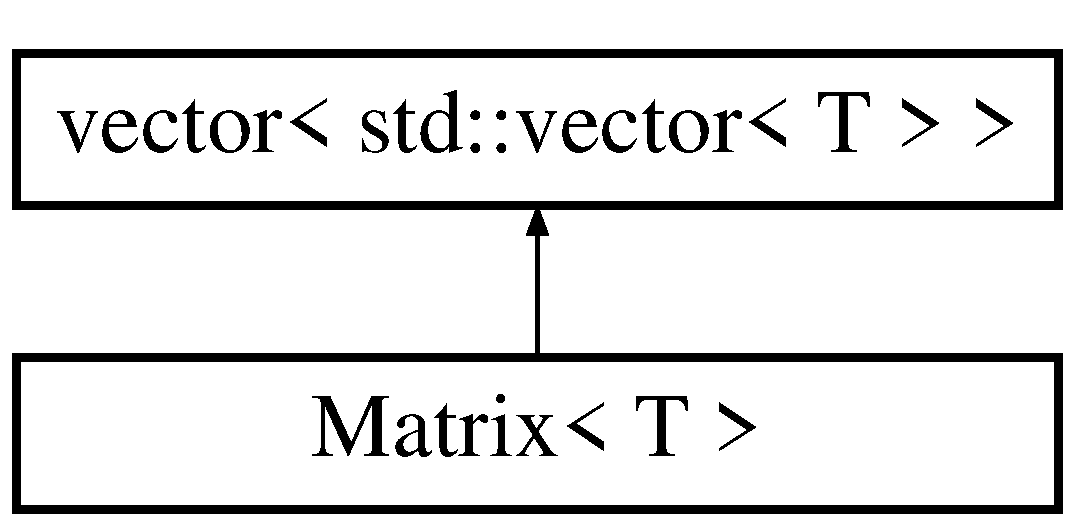
\includegraphics[height=2cm]{classMatrix}
\end{center}
\end{figure}
\subsection*{Public Methods}
\begin{CompactItemize}
\item 
{\bf Matrix} ()
\item 
{\bf Matrix} (const int \&)
\item 
{\bf Matrix} (const int \&, const int \&)
\item 
{\bf std::vector}$<$ T $>$ {\bf operator $\ast$} (const {\bf std::vector}$<$ T $>$ \&) const
\item 
{\bf std::vector}$<$ T $>$ {\bf get\-Column} (const int) const
\item 
Matrix$<$ T $>$ {\bf operator $\ast$} (const Matrix$<$ T $>$ \&) const
\item 
void {\bf print} ()
\end{CompactItemize}
\subsubsection*{template$<$class T$>$ class Matrix$<$ T $>$}



\subsection{Constructor \& Destructor Documentation}
\index{Matrix@{Matrix}!Matrix@{Matrix}}
\index{Matrix@{Matrix}!Matrix@{Matrix}}
\subsubsection{\setlength{\rightskip}{0pt plus 5cm}template$<$class T$>$ Matrix$<$ T $>$::Matrix ()}\label{classMatrix_a0}


\index{Matrix@{Matrix}!Matrix@{Matrix}}
\index{Matrix@{Matrix}!Matrix@{Matrix}}
\subsubsection{\setlength{\rightskip}{0pt plus 5cm}template$<$class T$>$ Matrix$<$ T $>$::Matrix (const int \&)}\label{classMatrix_a1}


\index{Matrix@{Matrix}!Matrix@{Matrix}}
\index{Matrix@{Matrix}!Matrix@{Matrix}}
\subsubsection{\setlength{\rightskip}{0pt plus 5cm}template$<$class T$>$ Matrix$<$ T $>$::Matrix (const int \&, const int \&)}\label{classMatrix_a2}




\subsection{Member Function Documentation}
\index{Matrix@{Matrix}!getColumn@{getColumn}}
\index{getColumn@{getColumn}!Matrix@{Matrix}}
\subsubsection{\setlength{\rightskip}{0pt plus 5cm}template$<$class T$>$ {\bf std::vector}$<$ T $>$ Matrix$<$ T $>$::get\-Column (const {\em int}) const}\label{classMatrix_a4}


\index{Matrix@{Matrix}!operator *@{operator $\ast$}}
\index{operator *@{operator $\ast$}!Matrix@{Matrix}}
\subsubsection{\setlength{\rightskip}{0pt plus 5cm}template$<$class T$>$ Matrix$<$ T $>$ Matrix$<$ T $>$::operator $\ast$ (const Matrix$<$ T $>$ \&) const}\label{classMatrix_a5}


\index{Matrix@{Matrix}!operator *@{operator $\ast$}}
\index{operator *@{operator $\ast$}!Matrix@{Matrix}}
\subsubsection{\setlength{\rightskip}{0pt plus 5cm}template$<$class T$>$ {\bf std::vector}$<$ T $>$ Matrix$<$ T $>$::operator $\ast$ (const {\bf std::vector}$<$ T $>$ \&) const}\label{classMatrix_a3}


\index{Matrix@{Matrix}!print@{print}}
\index{print@{print}!Matrix@{Matrix}}
\subsubsection{\setlength{\rightskip}{0pt plus 5cm}template$<$class T$>$ void Matrix$<$ T $>$::print ()}\label{classMatrix_a6}




The documentation for this class was generated from the following file:\begin{CompactItemize}
\item 
{\bf matrix.h}\end{CompactItemize}
